\scanpage{37}
\mspage{2}
\textcircled{\textcircled{e}}
\margin{$\varepsilon_0,\varepsilon_1$}
\[
\begin{gathered}
\sigma=\varepsilon_0\varepsilon_1\varepsilon_0=\varepsilon_1\varepsilon_0\varepsilon_1\\
\rho_0=(\varepsilon_1\varepsilon_0)^{-1},\quad\rho_1=(\varepsilon_0\varepsilon_1)^{-1}\\
\rho'_0=(\varepsilon_1\varepsilon_0)^2,\quad\rho'_1=(\varepsilon_0\varepsilon_1)^2
\end{gathered}
\]
\uuline{relation fondamentale}
\[
\boxed{\boxed{\begin{gathered}
\varepsilon_0\varepsilon_1\varepsilon_0=\varepsilon_1\varepsilon_0\varepsilon_1\qquad\text{ou}\\
\varepsilon_0\varepsilon_1\varepsilon_0\varepsilon_1^{-1}\varepsilon_0^{-1}\varepsilon_1^{-1}=1
\end{gathered}}}
\]
\textcircled{$f_0$}
\margin{$\sigma,\varepsilon_0$}
\[
\uline{\varepsilon_1=\sigma(\varepsilon_0)}=\sigma\varepsilon_0\sigma^{-1}
\]
\[
\boxed{\begin{aligned}\rho_0&=\sigma^{-1}\varepsilon_0\\\rho_1&=\varepsilon_0\sigma^{-1}\end{aligned}},\quad
\begin{aligned}\rho'_0&=\sigma\varepsilon_0\\\rho'_1&=\varepsilon_0\sigma\end{aligned}
\qquad
\boxed{\begin{gathered}[\sigma^2,\varepsilon_0]=1\\(\sigma^{-1}\varepsilon_0)^3=\sigma^{-2}\end{gathered}}
\]
Symétriques pour expression en $\sigma,\varepsilon_1$ (relations $f_1$)

\textcircled{\textcircled{$g_0$}}
\margin{$\sigma,\rho_0$}
\[
\begin{gathered}
\varepsilon_0=\sigma\rho_0,\quad\varepsilon_1=\rho_0\sigma\\
\rho'_0=\rho_0^{-2}\quad\deleted{\unsure{\rho_1}}\\
\rho_1=\sigma(\rho_0)=\sigma\rho_0\sigma^{-1}\\
\rho'_1=\sigma(\rho_0^{-2})=\sigma\rho_0^{-2}\sigma^{-1}
\end{gathered}
\qquad\boxed{\boxed{\underbrace{\rho_0^{-3}=\sigma^2}_{\omega}}}
\]
\deleted{élément central}\par
élément \deleted{\unsure{premier}}\unsure{univ.} central

Symétriques pour expression en $\sigma,\rho_1$, $\Leftarrow$ (relations $g_1$)

\textcircled{$g'_0$}
\margin{$\sigma,\rho'_0$}
\[
\begin{gathered}
\varepsilon_0=\sigma^{-1}\rho'_0\\
\varepsilon_1=\rho'_0\sigma^{-1}\\
\rho_0=\sigma^{-2}\rho'_0\\
\rho_1=\sigma^{-1}\rho'_0\sigma^{-1}=\\
\rho'_1=\sigma\rho'_0\sigma^{-1}
\end{gathered}
\qquad\boxed{\begin{gathered}[\sigma^2,\rho'_0]=1\quad\text{et}\\\rho_0'{}^3=\sigma^4\end{gathered}}
\]
Symétriques pour expression en $\sigma,\rho'_1$ (relations $g'_1$)

\textcircled{$h_0$}
\margin{$\varepsilon_0,\rho_0$}
\[
\begin{gathered}
\varepsilon_1=\rho_0(\varepsilon_0)=\rho_0\varepsilon_0\rho_0^{-1}\\
\sigma=\varepsilon_0\rho_0^{-1}\\
\rho'_0=\rho_0^{-2}\\
\rho_1=\varepsilon_0(\rho_0)=\varepsilon_0\rho_0\varepsilon_0^{-1}\\
\rho'_1=\varepsilon_0(\rho_0^{-2})=\varepsilon_0\rho_0^{-1}\varepsilon_0^{-1}
\end{gathered}
\]
\figure{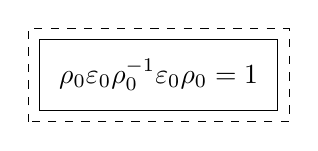
\begin{tikzpicture}\node[draw,inner sep=7pt] (r) {$\rho_0\varepsilon_0\rho_0^{-1}\varepsilon_0\rho_0=1$};\draw[dashed] ([xshift=-4pt,yshift=-4pt]r.south west) rectangle ([xshift=4pt,yshift=4pt]r.north east);\end{tikzpicture}}
Symétriques pour expression en $\varepsilon_1,\rho_1$ (relations $h_1$)
\margin{(à revoir!)}
\mspage{36}
